\section{Implementace aplikace}
Pro uživatelsky přívětivé ovládání systému bez potřeby přímého přístupu k serveru byla vyvinuta základní webová aplikace ve stylu SPA, tedy Single Page Application. Jde o druh webové aplikace, jejíž základ je popaán jen jediným webovým dokumentem a veškerý zbytek dat aplikace je načítán aplikací samotnou bez potřeby opakovaného načtení dokumentu\cite{SPASinglepageApplication2023}. Samotná aplikace je distribuována jako sada statických souborů a lze ji tak hostovat kdekoliv, včetně lokálního serveru. Dynamická data získává aplikace skrze REST API služby Facade, podobně jako jakýkoliv jiný samostatný klient.

Za základní framework, na kterém je aplikace postavena, bylo zvoleno Vue 3, které svou syntaxí připomíná framework Svelte, který je již používaný ve školním systému Kelvin \cite{SPASinglepageApplication2023}. Pro zjednodušení tvorby uživatelského rozhraní jsem použil komponentový framework Quasar\cite{QuasarframeworkQuasar2024}. Ten jsem zvolil po srovnání s jinými dostupnými Vue frameworky. Quasar jako jediný nabídl komponentu pro interakci se stromovitými daty, nevyžadoval žádné stylování ze strany vývojáře a měl dostatečně aktivní vývoj a komunitu. Jmenovitě jsem mimo Quasar evaluoval i Shadcn\cite{RadixvueRadixvue2024}, Vuetify\cite{VuetifyjsVuetify2024}, PrimeVue\cite{PrimefacesPrimevueNext}, Naive UI\cite{TusenaiNaiveui2024} a Radix Vue\cite{RadixvueShadcnvue2024}.

\subsection{Použité nástroje}
\begin{itemize}
    \item editor: WebStorm
    \item jazyk: TypeScript
    \item klient API: openapi-generator\cite{OpenAPIToolsOpenapigeneratorOpenAPI}
    \item knihovny:
        \begin{itemize}
            \item Reaktivita --> Vue\cite{VuejsCore2024}
            \item UI komponenty --> Quasar\cite{QuasarframeworkQuasar2024}
        \end{itemize}
\end{itemize}

\subsection{Struktura projektu}
\begin{itemize}
    \item assets/
        \begin{itemize}
            \item obsahuje soubory CSS stylů aplikace a případně soubory jako obrázky, fonty
        \end{itemize}
    \item components/
        \begin{itemize}
            \item obsahuje ,,hloupé'' komponenty, které nemají žádnou logiku a slouží jen k zobrazení dat
        \end{itemize}
    \item composables/
        \begin{itemize}
            \item obsahuje tzv. ,,composable'' funkce, které slouží k sdílení logiky mezi komponentami
        \end{itemize}
    \item layouts/
        \begin{itemize}
            \item obsahuje komponenty pro sdílení struktury stránek
        \end{itemize}
    \item router/
        \begin{itemize}
            \item obsahuje konfiguraci routeru aplikace a definice cest
        \end{itemize}
    \item services/
        \begin{itemize}
            \item obsahuje služby pro komunikaci s API
        \end{itemize}
    \item utils/
        \begin{itemize}
            \item obsahuje ruzné pomocné funkce
        \end{itemize}
    \item views/
        \begin{itemize}
            \item obsahuje komponenty pro jednotlivé obrazovky aplikace
        \end{itemize}
    \item App.vue
        \begin{itemize}
            \item hlavní komponenta aplikace
            \item obsahuje router-view a inicializaci uživatelova stavu
        \end{itemize}
    \item environment.ts
        \begin{itemize}
            \item obsahuje konfiguraci aplikace načtenou z proměnných prostředí
        \end{itemize}
    \item main.ts
        \begin{itemize}
            \item vstupní bod aplikace
            \item inicializace Vue aplikace
            \item inicializace frameworku Quasar
            \item inicializace knihovny Pinia\cite{VuejsPinia2024}
        \end{itemize}
\end{itemize}

\subsection{API klient}
Kód klienta k Facade API byl vygenerován nástrojem openapi-generator organizace OpenAPI Tools. Specificky intergrovaný generátor typescript-axios. Ten dostává na vstupu OpenAPI specifikaci a generuje soubory typově bezpečného klienta s podporou autentizace, variabilní adresou serveru, nahrávání souborů a metodami pojmenovanými podle atributu \lstinline|operationId| uvedeným ve specifikaci pro každou cestu.

\subsubsection{Úpravy klienta}
Kód vygenerovaného klienta bylo potřeba upravit z důvodu limitace OpenAPI popisu adres uživatelských souborů. Nepodporuje totiž adresní parametry obsahující lomítka, nejde je tedy s její pomocí validně popsat. Vygenerovaný klient parametry adresy, správně, dle specifikace, escapuje funkcí \lstinline|encodeURIComponent|. Pro možnost zachování používání, jinak nezměněného, klienta, napsal jsem skript, který po generaci vyhledá a přepíše instance kódu escapující parametry \lstinline|path| z kódující funkce jen na běžné převedení na řetězec. Příloha \ref{src:input-getmetadata-openapi} ukazuje popis cesty \lstinline|GET /hosted/core/files/{path}| pomocí OpenAPI dokumentu. V příloze \ref{src:output-getmetadata-openapi} je potom vidět vygenerovaná funkce \lstinline|getContentMetadata|.

Při inicializaci je vytvořena instance HTTP klienta axios\cite{AxiosAxios2024}, které je předána kořenová adresa služby Facade. Autentizační token je generovaným klientem načítán při každém požadavku funkcí \lstinline|accessToken()|, stačí ji tedy naimplementovat vlastní funkcí, která token vytáhne z lokálního úložiště. Klient má pak vždy aktuální token.

\begin{lstlisting}[label=src:facade-client-init,caption={Inicializace Facade API klienta}]
const axiosInstance = axios.create({
	baseURL: FACADE_URL,
});
const apiConfig = new Configuration({
	accessToken: () => getToken() || '',
});
export const api = {
	auth: AuthApiFactory(apiConfig, undefined, axiosInstance),
	admin: AdminApiFactory(apiConfig, undefined, axiosInstance),
	hosted: HostedApiFactory(apiConfig, undefined, axiosInstance),
	panels: PanelsApiFactory(apiConfig, undefined, axiosInstance),
	users: UsersApiFactory(apiConfig, undefined, axiosInstance),
	schedule: ScheduleApiFactory(apiConfig, undefined, axiosInstance),
};
\end{lstlisting}

Klient je umístěn ve vlastním balíčku \lstinline|facade-api-client| a je samostatně importovatelný.

\subsection{Ovládání aplikace}
Obrazovky aplikace pevně kopírují strukturu a funkcionalitu Facade API. Uživatel má možnost procházet seznamy uživatelů, panelů, úkolů a hostovaných souborů. Po výběru entity je uživatel přesměrován na obrazovku s detaily entity, kde je entita modifikovatelná. Po pozměnění dat entity je uživateli nabídnuto uložení změn a změny jsou odeslány na server.

\begin{figure}[h]
    \centering
    \subfloat[Obrazovka plánovaných úkolů (Desktop)\label{fig:eink-schedules-view}]{
        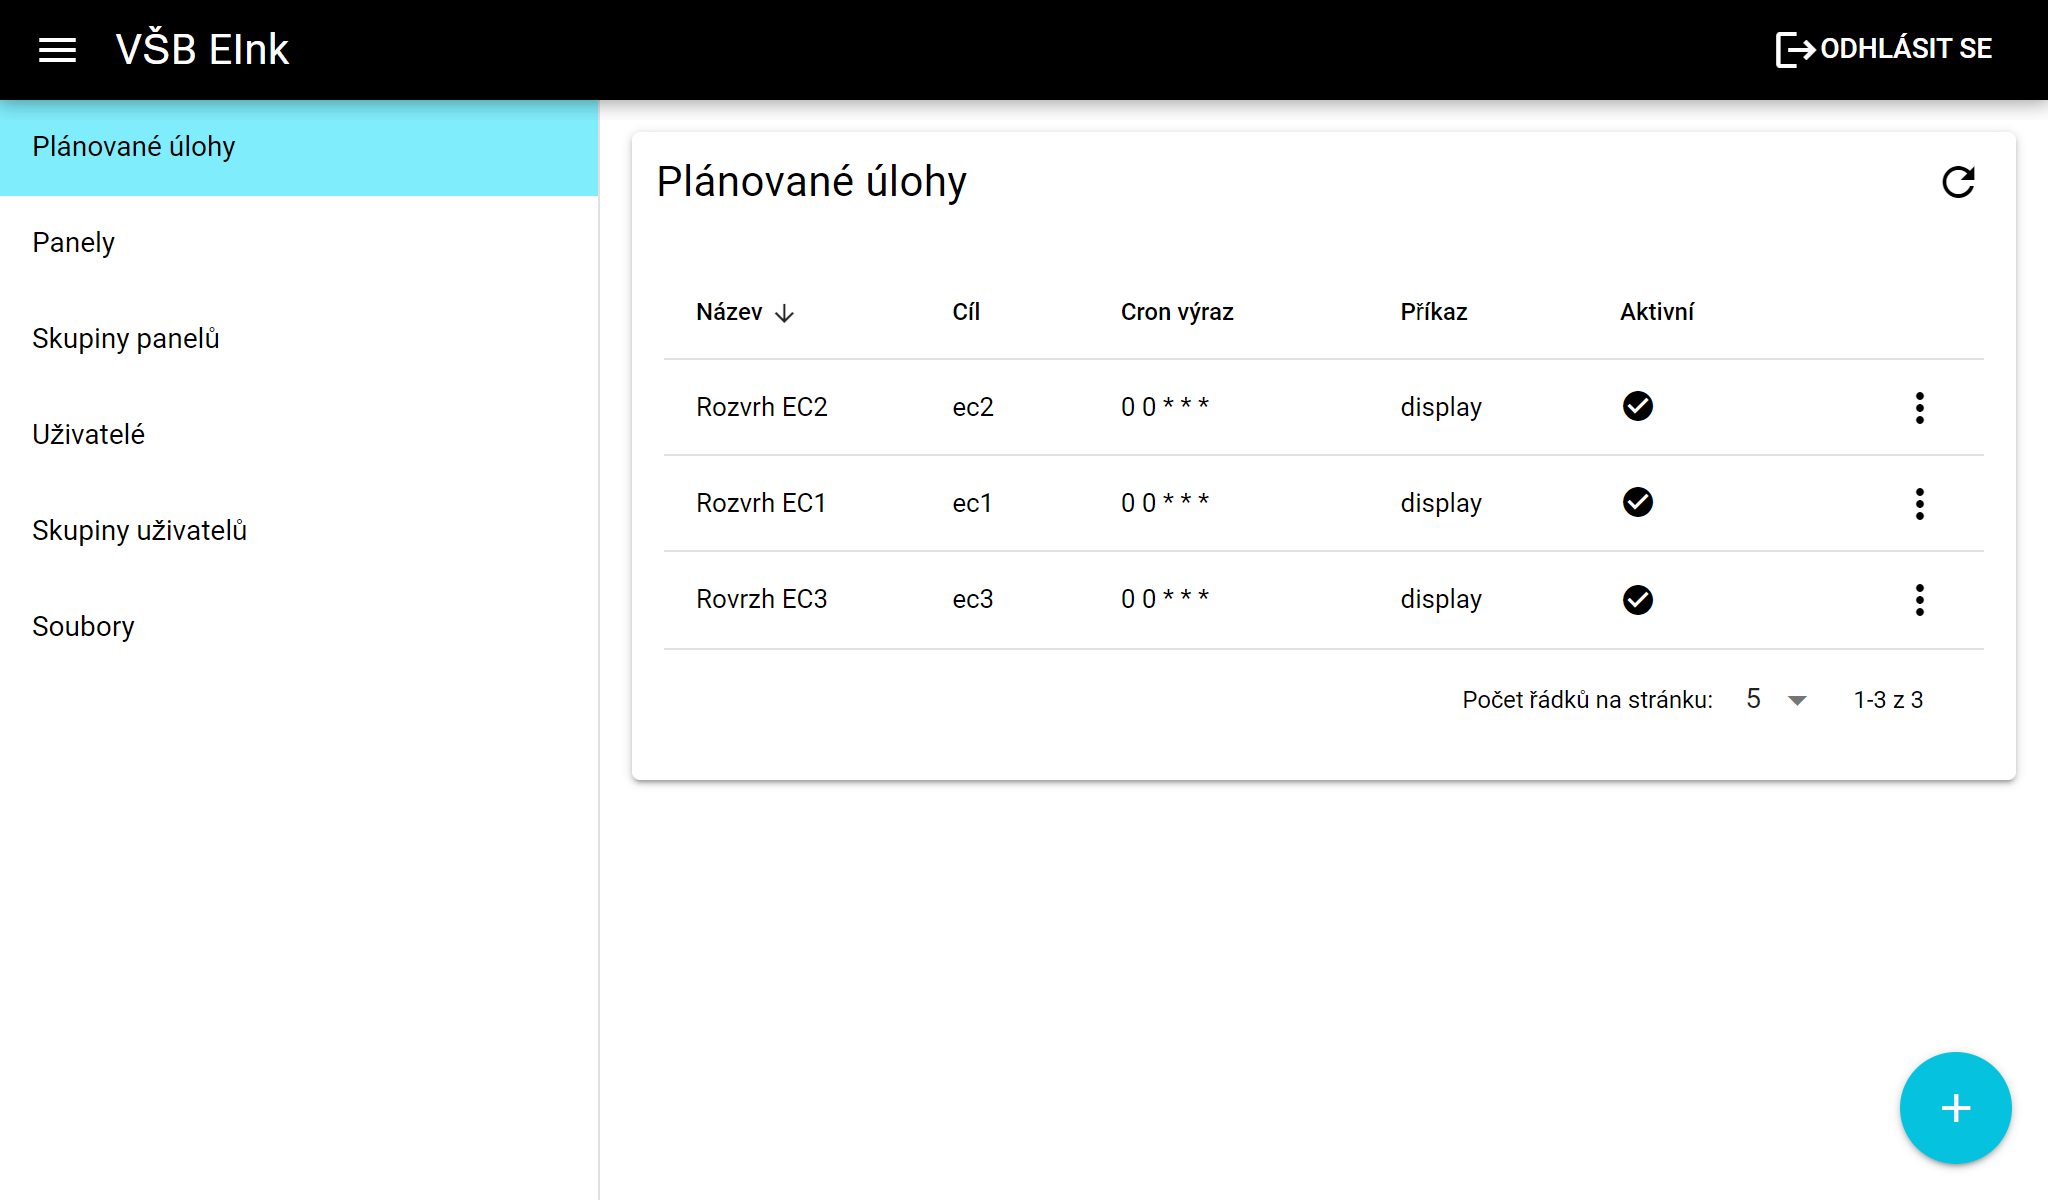
\includegraphics[width=0.70\textwidth]{Obrazky/aplikace/eink.a1314.cz_schedules.png}
    }
    \subfloat[Obrazovka plánovaných úkolů (Pixel 7)\label{fig:eink-schedules-pixel7-view}]{
        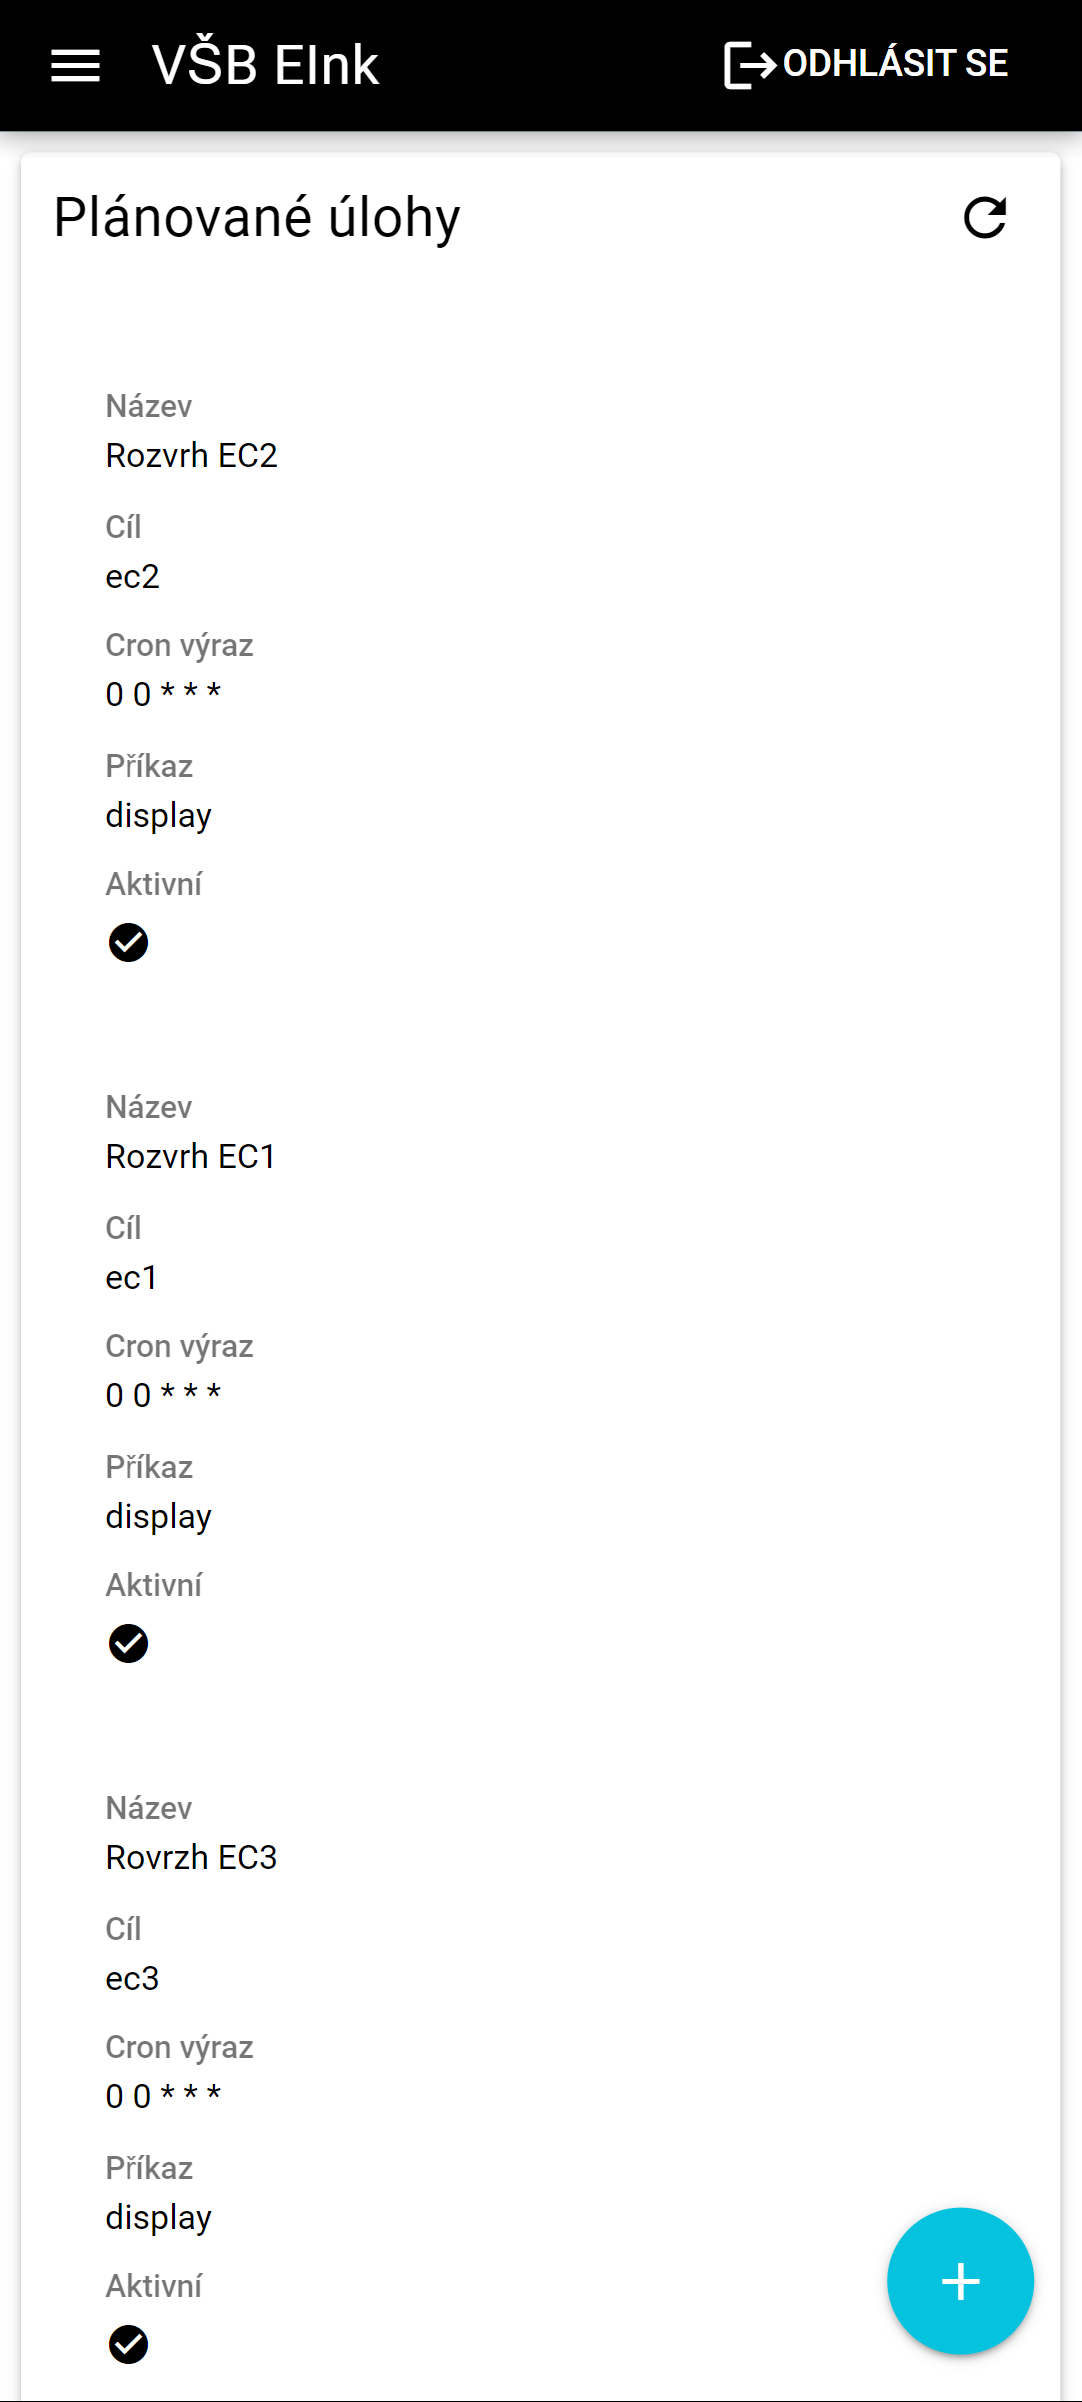
\includegraphics[width=0.28\textwidth]{Obrazky/aplikace/eink.a1314.cz_schedules_pixel7.png}
    }
    \caption{Srovnání obrazovek plánovaných úkolů na různých zařízeních}
	\label{fig:responsive-schedules}
\end{figure}
